\section{Analysis techniques}
\label{sec:method} 
We address imaging systematics in DESI data by performing a separate treatment for each imaging region (e.g., DECaLS North) within the DESI footprint to reduce the impact of systematic effects specific to that region. Once the imaging systematic weights are obtained for each imaging region separately, we combine the data from all regions to compute the power spectrum for the entire DESI footprint to increase the overall statistical power and enable more robust measurements of $\fnl$. We then conduct robustness tests on the combined data to assess the significance of any remaining systematic effects.


\subsection{Power spectrum estimator}
We first construct the density contrast field from the LRG density, $\rho$,
\begin{align}\label{eq:delta}
    \delta_{g} &= \frac{\rho- \overline{\rho}}{\overline{\rho}},
\end{align}
where the mean galaxy density $\overline{\rho}$ is estimated from the entire LRG sample. As a robustness test, we also analyze the power spectrum from each imaging region individually, in which $\overline{\rho}$ is calculated separately for each region. Then, we use the pseudo angular power spectrum estimator \citep{hivon2002master},
\begin{equation}\label{eq:pusedocell}
        \tilde{C}_{\ell} = \frac{1}{2\ell +1} \sum_{m=-\ell}^{\ell} |a_{\ell m}|^{2},
\end{equation}
where the coefficients $a_{\ell m}$ are obtained by decomposing $\delta_{g}$ into spherical harmonics, $Y_{\ell m}$,
\begin{equation}\label{eq:alm}
        a_{\ell m} = \int d\Omega ~ \delta_{g} W Y^{*}_{\ell m},
\end{equation}
where $W$ represents the survey window that is described by the number of randoms normalized to the expected value.

We use the implementation of \texttt{anafast} from the \textsc{HEALPix} package \citep{gorski2005healpix} to do fast harmonic transforms (Equation \ref{eq:alm}) and estimate the pseudo angular power spectrum of the LRG targets and the cross power spectrum between the LRG targets and the imaging systematic maps.

\subsection{Modelling}
The estimator in Equation \ref{eq:pusedocell} yields a biased power spectrum when the survey sky coverage is incomplete. Specifically, the survey mask causes correlations between different harmonic modes \citep{beutler2014clustering,wilson2017rapid}, and the measured clustering power is smoothed on scales near the survey size. An additional potential cause of systematic error arises from the fact that the mean galaxy density used to construct the density contrast field (Equation \ref{eq:delta}) is estimated from the available data, rather than being known a priori. This introduces what is known as an integral constraint effect, which can cause the power spectrum on modes near the size of the survey to be artificially suppressed, effectively pushing it towards zero \citep{peacock1991large,de2019integral}. Since $\fnl$ is highly sensitive to the clustering power on these scales, it is crucial to account for these systematic effects in the model galaxy power spectrum to obtain unbiased $\fnl$ constraints \citep[see, also,][]{riquelme2022primordial}, which we describe below.
  
The other theoretical systematic issues are however subdominant in the angular power spectrum. For instance, relativistic effects generate PNG-like scale-dependent signatures on large scales, which interfere with measuring $\fnl$ with the scale-dependent bias effect using higher order multipoles of the 3D power spectrum \citep{wang2020}. Similarly, matter density fluctuations with wavelengths larger than survey size, known as super-sample modes, modulate the galaxy 3D power spectrum \citep{castorina2020JCAP}. In a similar way, the peculiar motion of the observer can mimic a PNG-like scale-dependent signature through aberration, magnification and the Kaiser-Rocket effect, i.e., a systematic dipolar apparent blue-shifting in the direction of the observer's peculiar motion \citep{2021JCAP...11..027B}.
  
\subsubsection{Angular power spectrum} 
The relationship between the linear matter power spectrum $P(k)$ and the projected angular power spectrum of galaxies is expressed by the following equation:
\begin{equation}\label{eq:cell}
C_{\ell} = \frac{2}{\pi}\int_{0}^{\infty}\frac{dk}{k}k^{3}P(k)|\Delta_{\ell}(k)|^{2} + N_{\rm shot},
\end{equation}
where $N_{\rm shot}$ is a scale-independent shot noise term. The projection kernel $\Delta_{\ell}(k) = \Delta^{\rm g}_{\ell}(k) + \Delta^{\rm RSD}_{\ell}(k) + \Delta^{\mu}_{\ell}(k)$ includes redshift space distortions \mr{and magnification bias,} and determines the contribution of each wavenumber $k$ to the galaxy power spectrum on mode $\ell$. For more details on this estimator, refer to \cite{Padmanabhan2007}. The non-linearities in the matter power spectrum are negligible for the scales of interest \citep[see, e.g.,][]{Ho2015JCAP...05..040H}. For $\ell=40$, $\Delta_{\ell}(k)$ peaks at $k\sim 0.02~ h\text{Mpc}^{-1}$, which is above the non-linear regime. The FFTLog\footnote{\href{https://github.com/xfangcosmo/FFTLog-and-beyond}{github.com/xfangcosmo/FFTLog-and-beyond}} algorithm and its extension as implemented in \cite{fang2020beyond} are employed to calculate the integrals for the projection kernel $\Delta_{\ell}(k)$, which includes the $l^{\rm th}$ order spherical Bessel functions, $ j_{\ell}(kr)$, and its second derivatives,
\begin{align}
    \Delta^{\rm g}_{\ell}(k) &= \int \frac{dr}{r} r (b+\Delta b) D(r) \frac{dN}{dr} j_{\ell}(kr),\\
    \Delta^{\rm RSD}_{\ell}(k) &= - \int \frac{dr}{r} r f(r) D(r) \frac{dN}{dr} j^{\prime\prime}_{\ell}(kr),\\
    \Delta^{\mu}_{\ell}(k) &= - \ell(\ell+1) \int dr D(r) W_{\mu}(z) j_{\ell}(kr),
\end{align}
where $b$ is the linear bias (dashed curve in Figure \ref{fig:nz}), $D$ represents the linear growth factor normalized as $D(z=0)=1$, $f(r)$ is the growth rate, and $dN/dr$ is the redshift distribution of galaxies normalized to unity and described in terms of comoving distance\footnote{$dN/dr = (dN/dz)(dz/dr) \propto (dN/dz)H(z)$} (solid curve in Figure \ref{fig:nz}). \mr{The magnification bias window function $W_{\mu}(z)$ is}
\begin{equation}
W_{\mu}(z) = (5s-2)\frac{3H^{2}_{0}\Omega_{m}(1+z)}{2c^{2}k^{2}} \int_{z}^{\infty} dz^{\prime}\frac{dN}{dz} \frac{r(z^{\prime}) - r(z)}{r(z^{\prime})r(z)},
\end{equation}
\mr{where $\Omega_{m}$ is the matter density, $H_{0}$ is the Hubble constant\footnote{$H_{0}=100~({\rm km}~{\rm s}^{-1})/(h^{-1}{\rm Mpc})$ and $k$ is in unit of $h {\rm Mpc}^{-1}$}, $c$ is the speed of light, and $s$ is the response of the number density of galaxies to achromatic changes in the brightness. The parameter $s$ is estimated through shifting all magnitudes by an infinitesimal amount and re-running the color-mag selection. Our LRG targets are selected based on the fiber flux, whose response to magnification is different from the total flux and depends on the shape parameters for each morphology type \citep{zhou2023desi}. The parameter $s$ for our sample is found to vary slightly in the different imaging regions: $s=0.951\pm 0.011$ for BASS+MzLS, $s=0.943 \pm 0.007$ for DECaLS North+DECaLS South, and $s=0.945\pm 0.006$ for DESI\footnote{Private communication with Dr. Rongpu Zhou.}. We fix $s$ to the central values in our analysis.} The PNG-induced scale-dependent shift is given by \citep{slosar2008constraints}
\begin{equation}
\Delta b = b_{\phi}(z) \fnl \frac{3 \Omega_{m} H^{2}_{0}}{2 k^{2}T(k)D(z) c^{2}} \frac{g(\infty)}{g(0)},
\label{eq:scaledepbias}
\end{equation}
where $T(k)$ is the transfer function, and $g(\infty)/g(0) \sim 1.3$ with $g(z)\equiv (1+z) D(z)$ is the growth suppression due to non-zero $\Lambda$ because of our normalization of $D$ \citep[see, e.g.,][]{2010JCAP...07..013R, 2019MNRAS.485.4160M}. We assume the universality relation which directly relates $b_\phi$ to $b$ via $b_{\phi} = 2 \delta_{c}(b - p)$ with $\delta_{c}= 1.686$ representing the critical density for spherical collapse \citep{fillmore1984self}. We fix $p=1$ in our analysis and marginalize over b \citep[see, also,][]{slosar2008constraints,2010JCAP...07..013R,2013MNRAS.428.1116R}. 

\begin{figure}
\centering
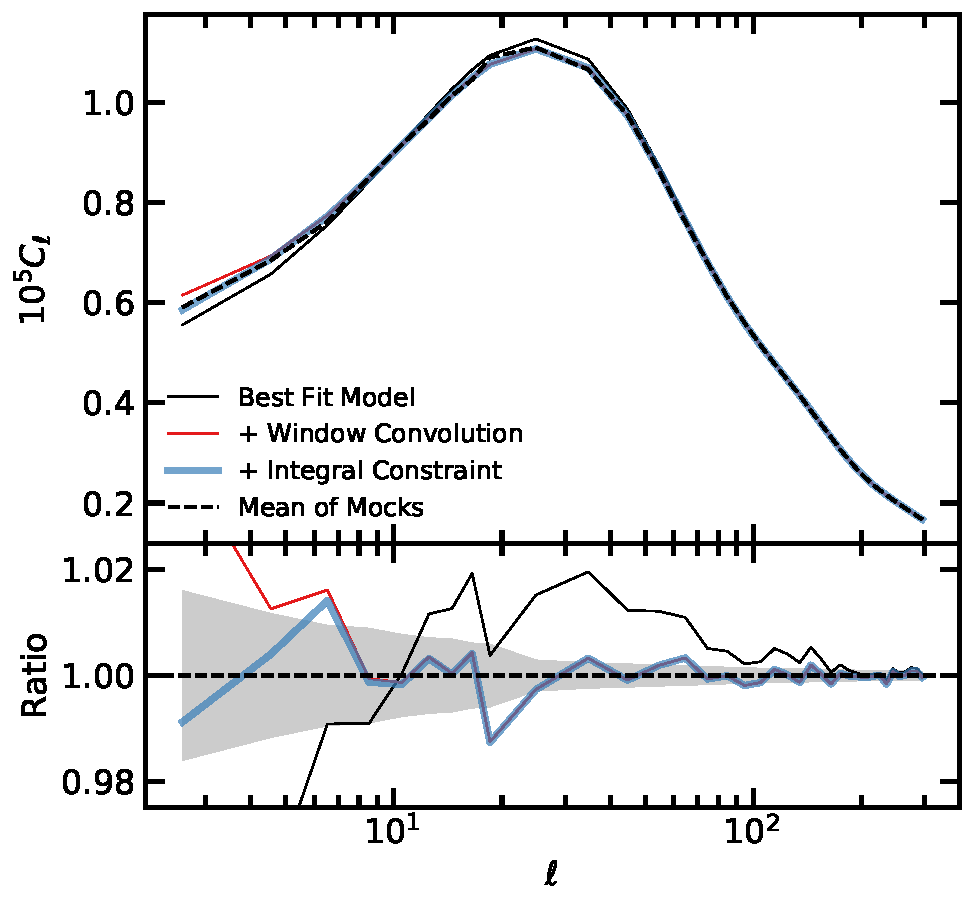
\includegraphics[width=0.45\textwidth]{model_mock.pdf}
\caption{The mean power spectrum from the $\fnl=0$ mocks (no contamination) and best-fitting theoretical prediction after accounting for the survey geometry and integral constraint effects. The dark and light shades represent the $68\%$ error on the mean and one realization, respectively. Bottom panel shows the residual power spectrum relative to the mean power spectrum. No imaging systematic cleaning is applied to these mocks.}\label{fig:model_mock}
\end{figure}

\subsubsection{Survey geometry and integral constraint}
We employ a technique similar to the one proposed by \cite{chon2004fast} to account for the impact of the survey geometry on the theoretical power spectrum. The ensemble average for the partial sky power spectrum is related to that of the full sky power spectrum via a mode-mode coupling matrix, ${\rm M}_{\ell \ell^{\prime}}$,
\begin{equation}\label{eq:mixm}
    <\tilde{C}_{\ell}> = \sum_{\ell^{\prime}} {\rm M}_{\ell \ell^{\prime}}<C_{\ell^{\prime}}>.
\end{equation}
We convert this convolution in the spherical harmonic space into a multiplication in the correlation function space. Specifically, we first transform the theory power spectrum (Equation \ref{eq:cell}) to the correlation function, $\hat{\omega}^{\rm model}$. Then, we estimate the survey mask correlation function, $\hat{\omega}^{\rm window}$, and obtain the pseudo-power spectrum,
\begin{align}
    \tilde{C}^{\rm model}_{\ell} &= 2\pi \int \hat{\omega}^{\rm model}\hat{\omega}^{\rm window}~P_{\ell}(\cos\theta) d\cos\theta.
\end{align}
\mr{Figure \ref{fig:mask2pf} illustrates ${\hat \omega}^{\rm window}$ for the different masks representing the DESI footprint and its imaging sub-regions. The smaller the region the sooner the mask correlation drops to zero (see \textit{area} in Table \ref{tab:imaging}).} The integral constraint is another systematic effect which is induced since the mean galaxy density is estimated from the observed galaxy density, and therefore is biased by the limited sky coverage \citep{peacock1991large}. To account for the integral constraint, the survey mask power spectrum is used to introduce a scale-dependent correction factor that needs to be subtracted from the power spectrum as,
\begin{equation}
     \tilde{C}^{\rm model, IC}_{\ell} = \tilde{C}^{\rm model}_{\ell} - \tilde{C}^{\rm model}_{\ell=0} \left(\frac{\tilde{C}^{\rm window}_{\ell}}{\tilde{C}^{\rm window}_{\ell=0}}\right),
\end{equation}
where $\tilde{C}^{\rm window}$ is the survey mask power spectrum, i.e., the spherical harmonic transform of $\hat{\omega}^{\rm window}$.

\begin{figure}
    \centering
    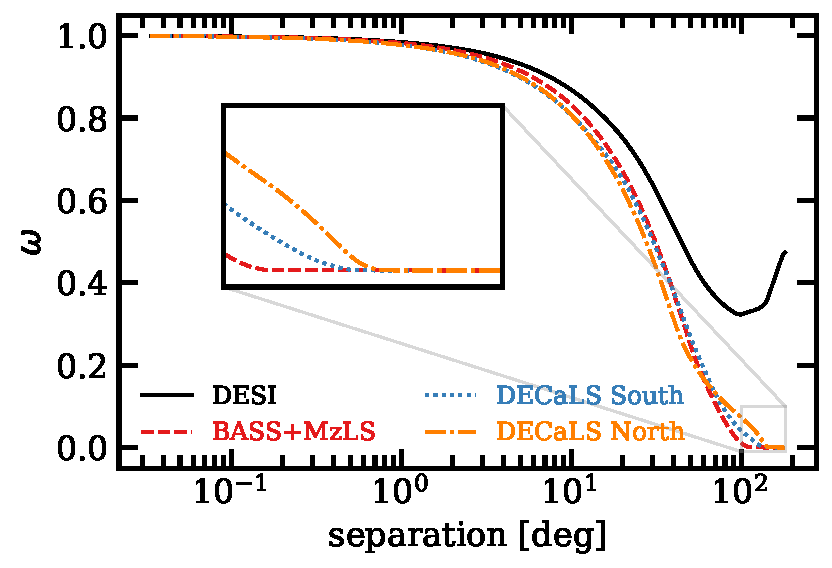
\includegraphics[width=0.45\textwidth]{figures/mask_2pf.pdf}
    \caption{\mr{The survey mask correlation functions for the imaging regions forming the DESI footprint as a function of angular separation. The inset shows the correlations specifically for angles between $100$ and $180$ degrees.}}
    \label{fig:mask2pf}
\end{figure}



The lognormal simulations are used to validate our survey window and integral constraint correction. Figure \ref{fig:model_mock} shows the mean power spectrum of the $\fnl=0$ simulations (dashed) and the best-fitting theory prediction before and after accounting for the survey mask and integral constraint. The simulations are neither contaminated nor mitigated. The light and dark shades represent the 68\% estimated error on the mean and one single realization, respectively. The DESI mask, which covers around $40\%$ of the sky, is applied to the simulations. We find that the survey window effect modulates the clustering power on $\ell < 200$ and the integral constraint alters the clustering power on $\ell < 6$.

\subsection{Parameter estimation}

\begin{figure*}
\centering
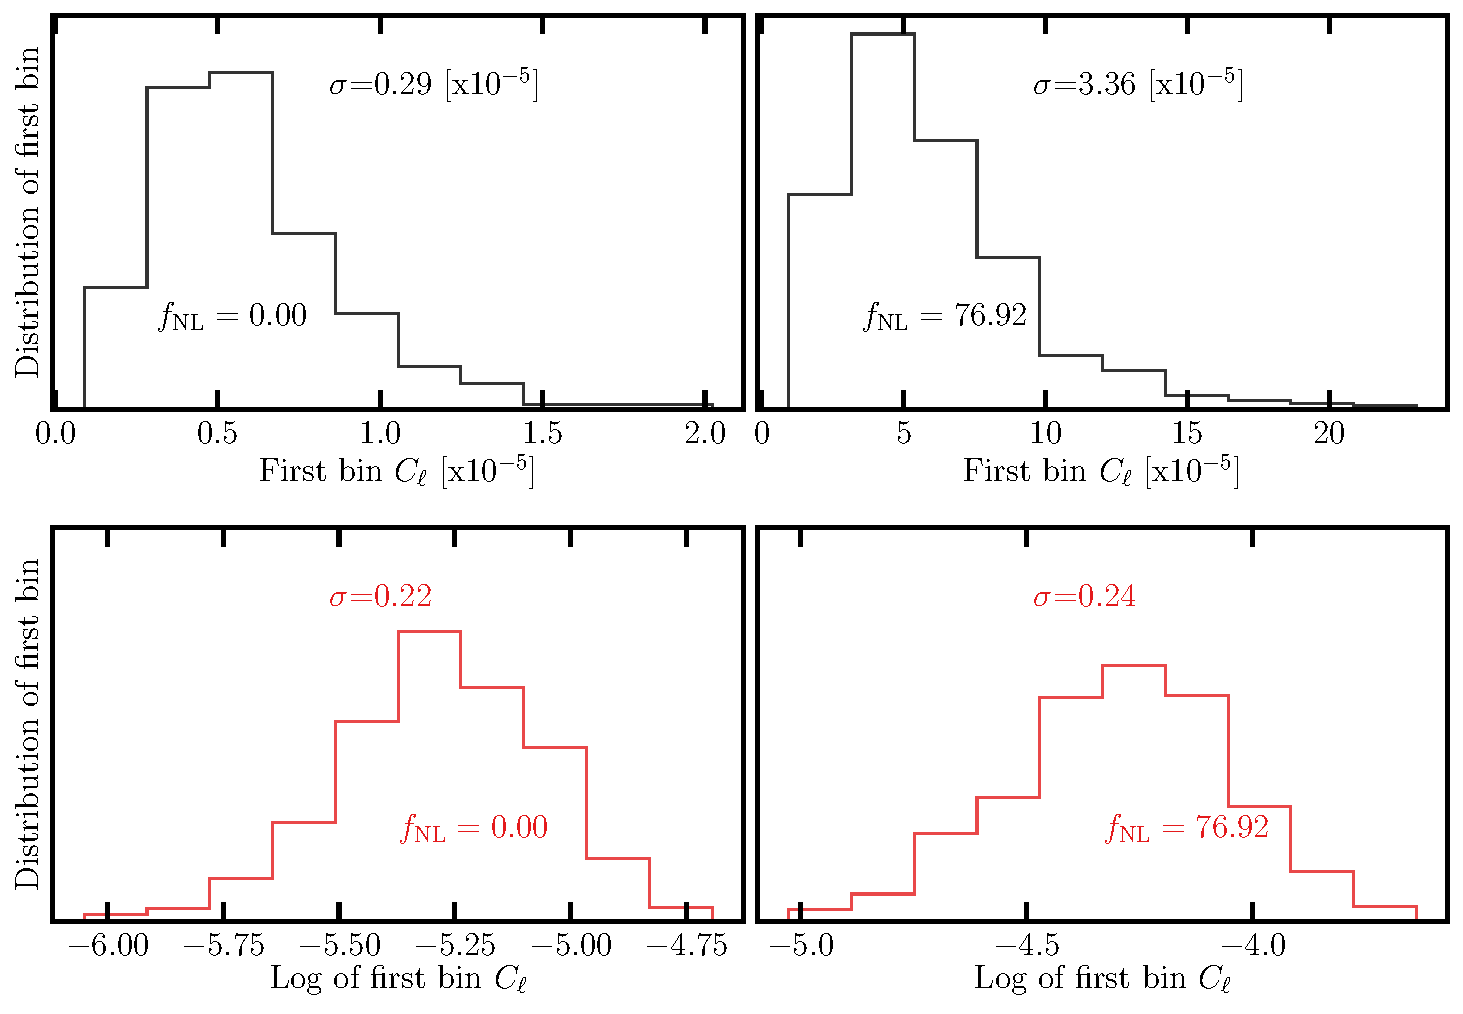
\includegraphics[width=0.85\textwidth]{hist_cl.pdf}
\caption{The distribution of the first bin power spectra and its log transformation from the simulations with $\fnl=0$ (left) and $76.9$ (right). The log transformation largely removes the asymmetry in the distributions.}\label{fig:histcell}
\end{figure*}

Our parameter inference uses standard MCMC sampling. A constant clustering amplitude is assumed to determine the redshift evolution of the linear bias of our DESI LRG targets, $b(z) = b/D(z)$, which is supported by the HOD fits to the angular power spectrum \citep{zhou2021clustering}. In MCMC, we allow $\fnl$, $N_{\rm shot}$, and $b$ to vary, while all other cosmological parameters are fixed at the fiducial values (see \S \ref{ssec:mocks}). The galaxy power spectrum is divided into a discrete set of bandpower bins with $\Delta\ell=2$ between $\ell=2$ and $20$ and $\Delta \ell=10$ from $\ell=20$ to $300$. Each clustering mode is weighted by $2\ell+1$ when averaging over the modes in each bin.

The expected large-scale power is highly sensitive to the value of $\fnl$ such that the the amplitude of the covariance for $C_{\ell}$ is influenced by the true value of $\fnl$, see also \cite{2013MNRAS.428.1116R} for a discussion. As illustrated in the top row of Figure \ref{fig:histcell}, we find that the distribution of the power spectrum at the lowest bin, $2\leq \ell < 4$, is highly asymmetric and its standard deviation varies significantly from the simulations with $\fnl=0$ to $76.9$. We can make the covariance matrix less sensitive to $\fnl$ by taking the log transformation of the power spectrum, $\log C_{\ell}$. As shown in the bottom panels in Figure \ref{fig:histcell}, the log transformation reduces the asymmetry and the difference in the standard deviations between the $\fnl=0$ and $76.9$ simulations. Therefore, we minimize the negative log likelihood defined as,
\begin{equation}\label{eq:likelihood}
-2\log \mathcal{L} = (\log \tilde{C}(\Theta)-\log \tilde{C})^{\dagger} \mathbb{C}^{-1} (\log \tilde{C}(\Theta)-\log \tilde{C}),
\end{equation}
where $\Theta$ represents a container for the parameters $\fnl$, $b$, and $N_{\rm shot}$; $\tilde{C}(\Theta)$ is the (binned) expected pseudo-power spectrum; $\tilde{C}$ is the (binned) measured pseudo-power spectrum; and $\mathbb{C}$ is the covariance on $\log\tilde{C}$ constructed from the $\fnl=0$ log-normal simulations. Log-normal simulations have been commonly used and validated to estimate the covariance matrices for galaxy density fields, and non-linear effects are subdominant on the scales of interest to $\fnl$ \citep[see, e.g.,][]{2017MNRAS.466.1444C, 2021MNRAS.508.3125F}. We also test for the robustness of our results against an alternative covariance constructed from the $\fnl=76.9$ mocks. Flat priors are implemented for all parameters: $\fnl \in [-1000, 1000]$, $N_{\rm shot} \in [-0.001, 0.001]$, and $b \in [0, 5]$.


\subsection{Characterization of remaining systematics}
\label{ssec:characterization}

One potential problem that can arise in the data-driven mitigation approach is \textit{over-correction}, which occurs when the corrections applied to the data remove the clustering signal and induce additional biases in the inferred parameter. The neural network approach is more prone to this issue compared to the linear approach due to its increased degrees of freedom. As illustrated in the bottom panel of Figure \ref{fig:pcc}, the significant correlations among the imaging systematic maps may pose additional challenges for modeling the spurious fluctuations in the galaxy density field. Specifically, using highly correlated imaging systematic maps increases the statistical noise in the imaging weights, which elevates the potential for over subtracting the clustering power. These over-correction effects are estimated to have a negligible impact on baryon acoustic oscillations \citep{merz2021clustering}; however, they can significantly modulate the galaxy power spectrum on large scales, and thus lead to biased $\fnl$ constraints \citep{rezaie2021primordial, mueller2022primordial}. Although not explored thoroughly, the over-correction issues could limit the detectability of primordial features in the galaxy power spectrum and that of parity violations in higher order clustering statistics \citep{beutler2019primordial, cahn2021test, philcox2022probing}. Therefore, it is crucial to develop, implement, and apply techniques to minimize and control over-correction in the hope of ensuring that the constraints are as accurate and reliable as possible; one such approach is to reduce the dimensionality of the problem. 

Our goal is to reduce the correlations between the DESI LRG target density and the imaging systematic maps while controlling the over-correction effect. Below, we describe how we achieve this objective, by employing a series of simulations along with the residual systematics that we construct based on the cross power spectrum between the LRG density and imaging maps, and the mean LRG density as a function of imaging. We test different sets of the imaging systematic maps to identify the optimal set of the feature maps:
\begin{enumerate}[itemindent=*]
\item \textbf{Two maps}: Extinction, depth in z.
\item \textbf{Three maps}: Extinction, depth in z, psfsize in r.
\item \textbf{Four maps}: Extinction, depth in z, psfsize in r, stellar density.
\item \textbf{Five maps}: Extinction, depth in z, psfsize in r, neutral hydrogen density, and photometric calibration in z.
\item \textbf{Eight maps}: Extinction, depth in $grzW1$, psfsize in $grz$.
\item \textbf{Nine maps}: Extinction, depth in $grzW1$, psfsize in $grz$, stellar density.
\end{enumerate}

\begin{figure*}
\centering
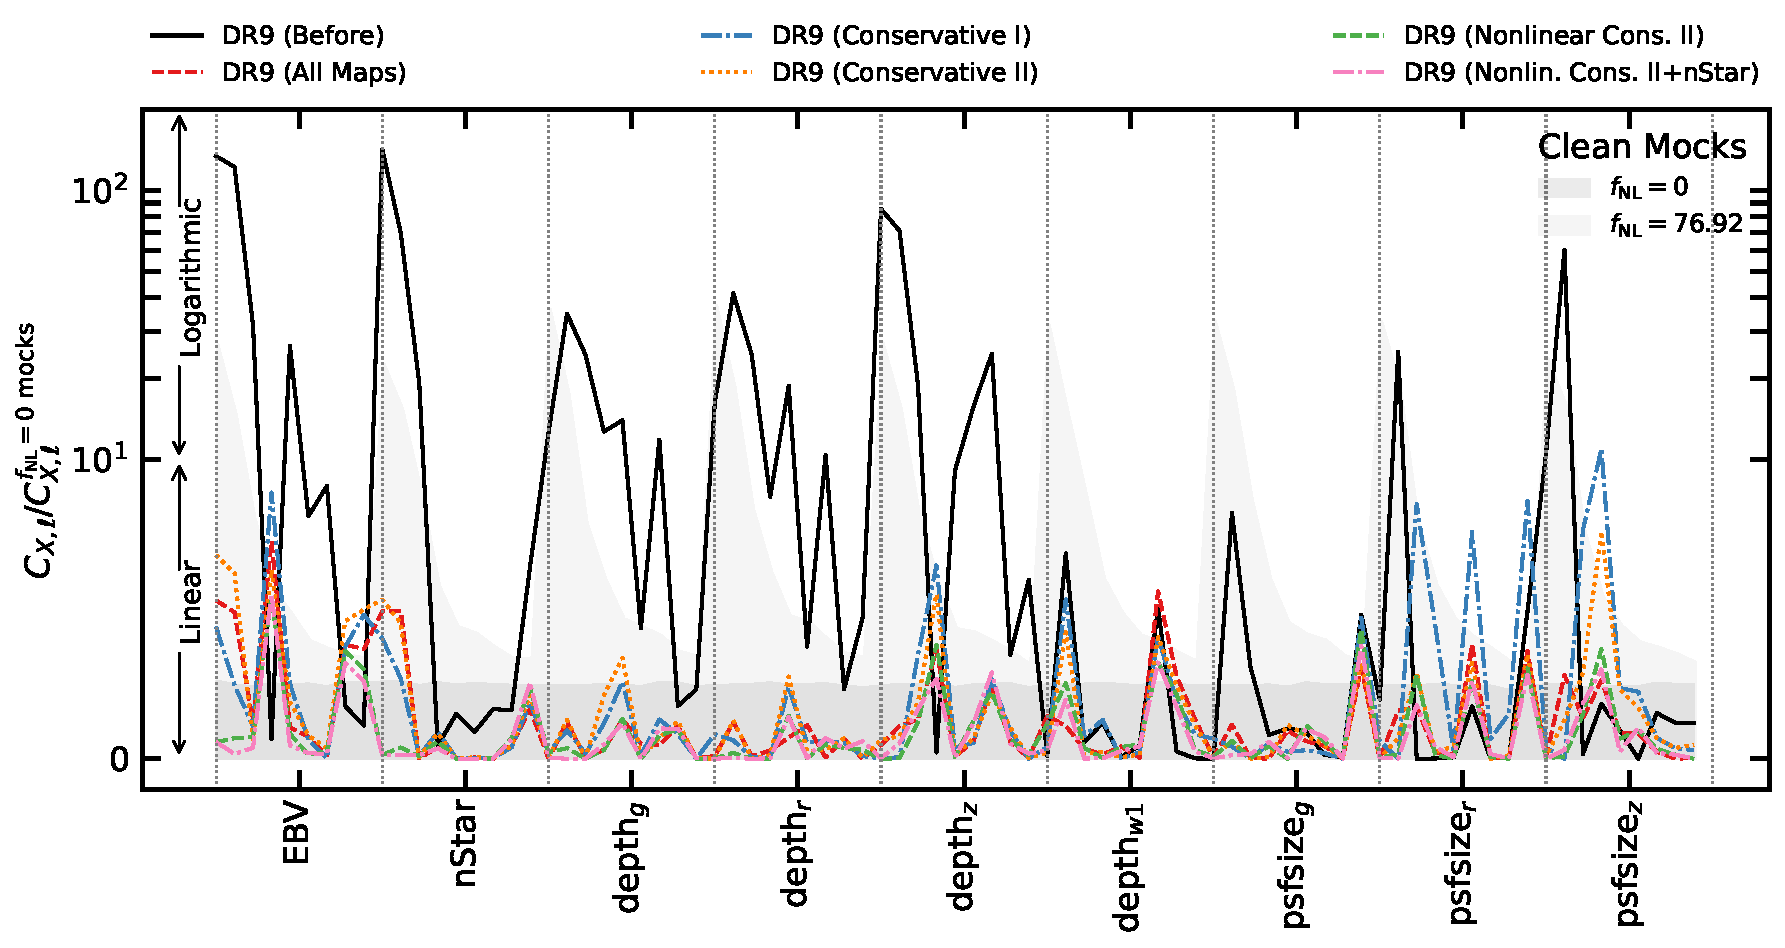
\includegraphics[width=0.95\textwidth]{clx_mocks.pdf}
\caption{The square of the cross power spectra between the DESI LRG targets and imaging systematic maps normalized by the auto power spectrum of the imaging systematic maps; see equation \ref{eq:cx}. The systematic maps considered are Galactic extinction (EBV), stellar density (nStar), depth in \textit{grzw1} (depth$_{grzw1}$), and seeing in \textit{grz} (psfsize$_{grz}$). The black curves display the cross spectra before imaging systematic correction. The red, blue and orange curves represent the results after applying the imaging weights from the linear models trained with \textit{eight maps}, \textit{two maps}, and \textit{three maps}. The green and pink curves display the results after applying the imaging weights from the nonlinear models trained with \textit{three maps} and \textit{four maps}. The dark and light shades represent the $97.5$ percentile from cross correlating the imaging systematic maps and the $\fnl=0$ and $76.9$ lognormal density fields, respectively.}\label{fig:clxmock}
\end{figure*}

It is imperative to note that these sets are selected prior to examining the auto power spectrum of the LRG sample and unblinding the $\fnl$ constraints, and that the auto power spectrum and $\fnl$ measurements are unblinded only after our mitigation methods passed our rigorous tests for residual systematics. 

\begin{figure*}
\centering
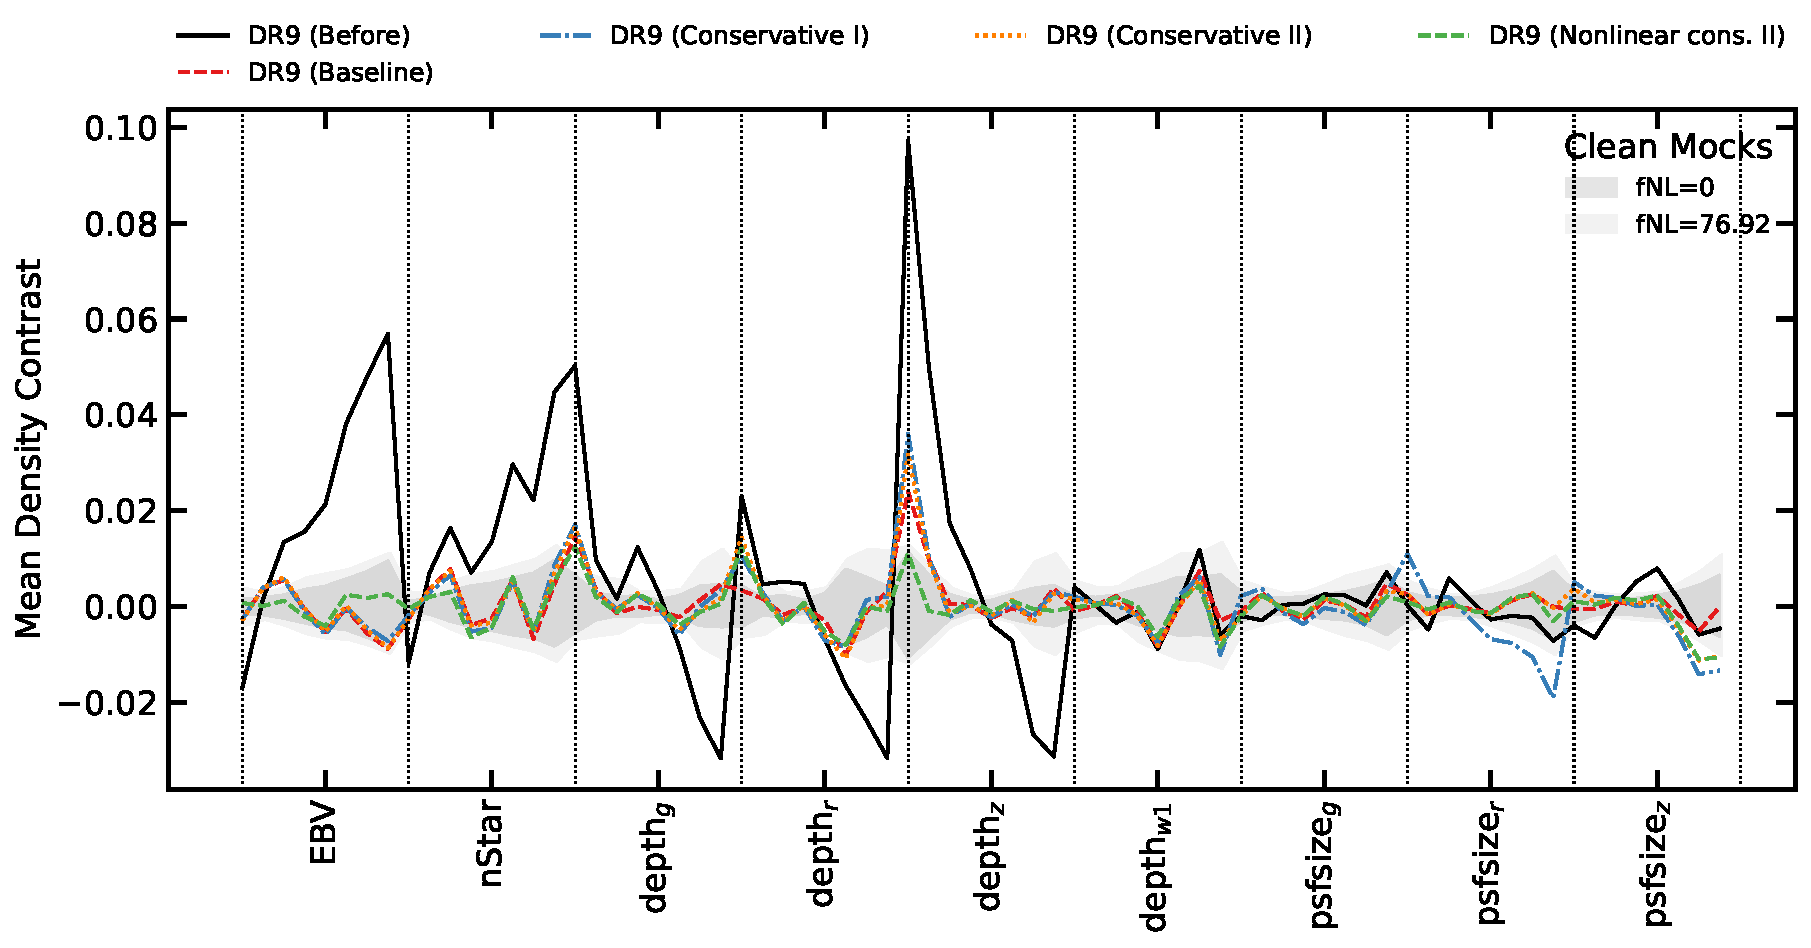
\includegraphics[width=0.95\textwidth]{nbar_mocks.pdf}
\caption{The mean density contrast of the DESI LRG targets as a function of the imaging systematic maps: Galactic extinction (EBV), stellar density (nStar), depth in \textit{grzw1} (depth$_{grzw1}$), and seeing in \textit{grz} (psfsize$_{grz}$). The black curves display the results before imaging systematic correction. The red, blue and orange curves represent the relationships after applying the imaging weights from the linear models trained with \textit{two maps}, \textit{three maps}, and \textit{eight maps}, respectively. The green and pink curves display the results after applying the imaging weights from the nonlinear models trained with \textit{three maps} and \textit{four maps}. The dark and light shades represent the $68\%$ dispersion of 1000 lognormal mocks with $\fnl=0$ and $76.9$, respectively.}\label{fig:nbarmock}
\end{figure*}


\begin{figure}
\raggedright
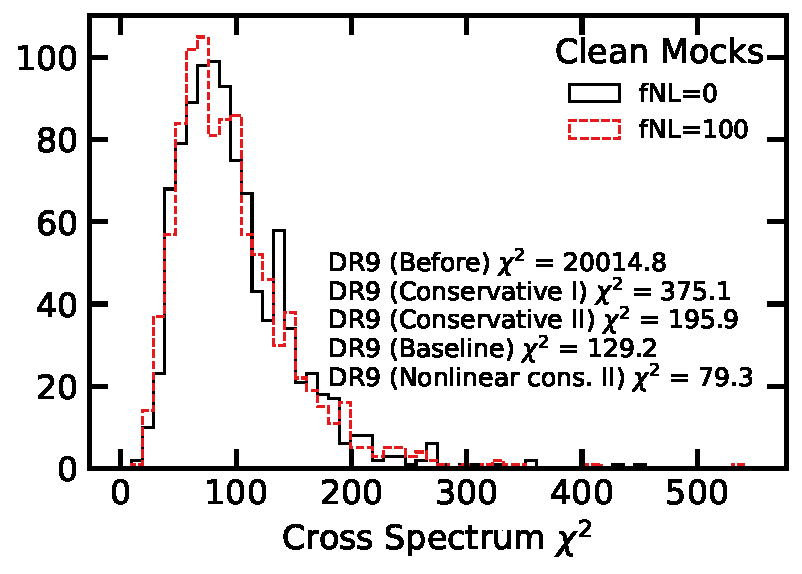
\includegraphics[width=0.45\textwidth]{chi2test.pdf}
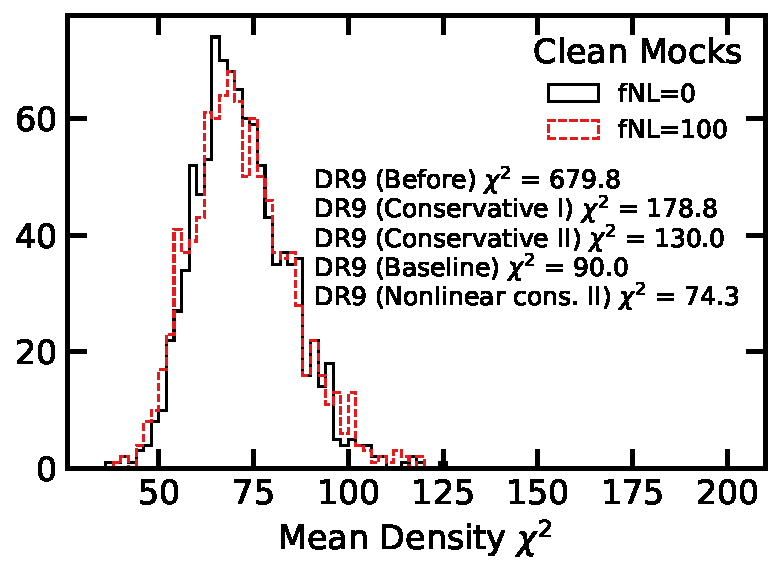
\includegraphics[width=0.44\textwidth]{chi2test2.pdf}
\caption{The remaining systematic error $\chi^{2}$ from the galaxy-imaging cross power spectrum (top) and the mean galaxy density contrast (bottom). The values observed in the DESI LRG targets before and after linear and nonlinear treatments are represented via vertical lines, and the histograms are constructed from 1000 realizations of clean lognormal mocks with $\fnl=0$ and $76.9$.}\label{fig:chi2test}
\end{figure}


\subsubsection{Cross power spectrum}

We characterize the cross correlations between the galaxy density and imaging systematic maps by
\begin{equation}
\tilde{C}_{X, \ell} = [\tilde{C}_{x_{1}, \ell}, \tilde{C}_{x_{2}, \ell}, \tilde{C}_{x_{3}, \ell}, ..., \tilde{C}_{x_{9}, \ell}],
\end{equation}
where $\tilde{C}_{x_{i}, \ell}$ represents the the square of the cross power spectrum between the galaxy density and $i^{\rm th}$ imaging map, $x_{i}$, divided by the auto power spectrum of $x_{i}$:
\begin{equation}\label{eq:cx}
\tilde{C}_{x_{i}, \ell} = \frac{(\tilde{C}_{gx_{i}, \ell})^{2}}{\tilde{C}_{x_{i}x_{i},\ell}}.
\end{equation}
With this normalization, $\tilde{C}_{x_{i}, \ell}$ estimates the contribution of systematics at every multipole up to the linear order to the galaxy power spectrum. Then, the $\chi^{2}$ value for the cross power spectra is calculated via,
\begin{equation}\label{eq:cx_chi2}
\chi^{2} = \tilde{C}^{T}_{X, \ell} \mathbb{C}_{X}^{-1} \tilde{C}_{X, \ell},
\end{equation}
where the covariance matrix $\mathbb{C}_{X} = < \tilde{C}_{X, \ell} \tilde{C}_{X, \ell'} >$ is constructed from the lognormal mocks. These $\chi^{2}$ values are measured for every clean mock realization with the \textit{leave-one-out} technique and compared to the values observed in the LRG sample with various imaging systematic corrections. Specifically, we use 999 realizations to estimate a covariance matrix and then apply the covariance matrix from the 999 realizations to measure the $\chi^{2}$ for the one remaining realization. This process is repeated for all 1000 realizations to construct a histogram for $\chi^{2}$. We only include the bandpower bins from $\ell=2$ to $20$ with $\Delta\ell=2$, and test for the robustness with higher $\ell$ modes in Appendix \ref{sec:scalesys}. 

We identify extinction and depth in the z band as two primary potential contaminants, and run the linear model with these two maps to derive the systematic weights. Linear two maps is the most conservative systematic treatment method in terms of both the model flexibility and the number of input maps. We clean the sample using the imaging weights obtained from \textit{linear two maps}, and find that the linear two maps approach mitigates most of the spurious density fluctuations and reduces the cross-correlations between the LRG density and the imaging systematic maps, except for the trends against psfsize in the r and z bands. Adding the r-band psfsize improves the linear model performance such that the cross correlations are similar to those obtained from \textit{linear eight maps}, which indicates no further information can be extracted from eight maps. Therefore, we identify extinction, depth in z, and psfsize in r (\textit{three maps}) as the primary sources of systematic effects in the DESI LRG targets. Then, we adapt \textit{neural network three maps} to model non-linear systematic effects. Compared with the linear three maps method, we find that the neural network-based weights significantly reduce the cross correlations and spurious density fluctuations of the DESI LRG sample and imaging systematic maps. Additionally, we consider neural networks with four, five, and nine maps to further examine the robustness of our cleaning methods. Figure \ref{fig:clxmock} shows $\tilde{C}_{X}$ from the DESI LRG targets before and after applying various corrections for imaging systematics. The dark and light shades show the 97.5$^{\rm th}$ percentile from the $\fnl=0$ and $76.9$ mocks, respectively. Without imaging weights, the LRG sample has the highest cross-correlations against extinction, stellar density, and depth in z (solid black curve). There are less significant correlations against depth in the g and r bands, and psfsize in the z band, which could be driven because of the inner correlations between the imaging systematic maps. First, we consider cleaning the sample with the linear model using two maps (extinction and depth in z) as identified from the Pearson correlation. With linear two maps (red dashed curve), most of the cross power signals are reduced below statistical uncertainties, especially against extinction, stellar density, and depth. However, the cross power spectra against psfsize in r and z increases slightly on $6<\ell<20$ and $6<\ell<14$, respectively. Regression against extinction and depth in the z-band helps mitigate large-scale cross correlations ($\ell < 6$), but there are some residual cross correlations on smaller scales ($\ell > 6$) which cannot be mitigated with our set of two maps. The linear three maps (blue dot-dashed curve) approach alleviates the cross power spectrum against psfsize in r. Additionally, nonlinear three maps (green dashed curve) can reduce the cross correlations against both the r and z-band psfsize maps, which shows the benefit of using a nonlinear approach. For benchmark, we also show the normalized cross spectra after cleaning the LRG sample with linear eight maps (orange dotted curve) and nonlinear four maps (pink dot-dashed curve). 

\subsubsection{Mean density contrast}
We calculate the histogram of the mean density contrast relative to the $j^{\rm th}$ imaging property, $x_{j}$:
\begin{equation}
\delta_{x_{j}} = ({\overline{\rho}})^{-1} \frac{\sum_{i} \rho_{i} W_{i}}{\sum_{i} W_{i}} \mr{- 1},
\end{equation}
where $\overline{\rho}$ is the global mean galaxy density, $W_{i}$ is the survey window in pixel $i$, and the summations over $i$ are evaluated from the pixels in every bin of $x_{j}$. We compute the histograms against all nine imaging properties (see Figure \ref{fig:ng}). We use a set of eight equal-width bins for every imaging map, which results in a total of 72 bins. Then, we construct the total mean density contract as,
\begin{equation}
\delta_{X} = [\delta_{x_{1}}, \delta_{x_{2}}, \delta_{x_{3}}, ..., \delta_{x_{9}}],
\end{equation}
and the total residual error as,
\begin{equation}
\chi^{2} = \delta_{X}^{T} \mathbb{C_{\delta}}^{-1} \delta_{X},
\end{equation}
where the covariance matrix $\mathbb{C}_{\delta} = < \delta_{X} \delta_{X}>$ is constructed from the lognormal mocks. Figure \ref{fig:nbarmock} shows the mean density contrast against the imaging properties for the DESI LRG targets. The dark and light shades represent the $1\sigma$ level fluctuations observed in 1000 lognormal density fields respectively with $\fnl=0$ and $76.9$. The DESI LRG targets before treatment (solid curve) exhibits a strong trend around $10\%$ against the z-band depth which is consistent with the cross power spectrum. Additionally, there are significant spurious trends against extinction and stellar density at about $5-6\%$. The linear approach is able to mitigate most of the systematic fluctuations with only extinction and depth in the z-band as input; however, a new trend appears against the r-band psfsize map with the \textit{linear two maps} approach (red dashed curve), which is indicative of the psfsize-related systematics in our sample. This finding is in agreement with the cross power spectrum. We re-train the linear model with three maps, but we still observe around $2\%$ residual spurious fluctuations in the low end of depth$_{z}$ and around $1\%$ in the high end of psfsize$_{z}$, which implies the presence of nonlinear systematic effects. We find that the imaging weights from the nonlinear model trained with the three identified maps (or four maps including the stellar density) are capable of reducing the fluctuations below $2\%$. Even with the nonlinear three maps, we have about $1\%$ remaining systematic fluctuations against the z-band psfsize. We use the $\chi^{2}$ statistics to assess how significant these fluctuations are in comparison to the clean mocks. 

Figure \ref{fig:chi2test} presents $\chi^{2}$ histograms for the normalized cross spectrum (top) and mean density contrast (bottom) statistics obtained from lognormal mocks with different $\fnl$ values. The $\chi^{2}$ tests are insensitive to $\fnl$, providing consistent distributions regardless of its value that was used for mock generation, and thus these tests help separate systematics from cosmology. No mitigation is applied to the mocks, ensuring unbiased $\chi^{2}$ values. DESI LRG target $\chi^{2}$ values are compared via the vertical lines and summarized in Table \ref{tab:chi2test}.

After cleaning, the cross power spectrum's $\chi^{2}$ is reduced. However, linear three maps approach fails to clean the data properly at $95\%$ confidence ($\chi^{2}=195.9$ and $p$-value $< 0.04$). Alternative nonlinear three maps approach reduces $\chi^{2}$ significantly with $p$-value$=0.59$, supporting the need for nonlinear cleaning. For this test, we only use multipoles for up to $\ell=20$, and we find no remaining systematic errors by investigating at higher multipoles (see Appendix \ref{sec:scalesys}). We observe similar performance in the mean density test. The \textit{linear two maps} weights reduce the $\chi^{2}$ from $679.8$ to $178.8$, but significant systematics remain ($p$-value $<0.001$). Applying the linear three maps approach lowers the error to $\chi^{2}=130$, yet systematics remain significant ($p$-value $<0.001$). Cleaning with linear eight maps results in $\chi^{2}=90$ and $p$-value $=0.08$, but using too many imaging maps increases the risk of removing the true clustering signal. Alternatively, using imaging weights from the \textit{nonlinear three maps} approach yields $\chi^{2}=74.3$ and $p$-value $=0.39$. Adding the stellar density map (\textit{nonlinear four maps}) slightly improves the results: $\chi^{2}=73.2$ and $p$-value $=0.42$. The small impact on $\chi^{2}$ suggests that the stellar density trend can be explained by extinction due to the correlation between these properties, such that in regions with high stellar density, there is likely to be a higher concentration of dust, which can cause greater extinction of light. \mr{The nonlinear method with nine maps is our most aggressive treatment which results in the lowest residual errors, $\chi^{2}=39.7$ ($p$-value = $>0.99$) and $49.1$ ($p$-value = $0.88$), respectively, for the mean density and cross-power spectrum statistics. The $p$-values are obtained from the comparison to the clean mocks that have had not mitigation applied to them. To assess whether the extra reduction in the $\chi^{2}$ (by using the extra maps in the non-linear nine maps) indicates over-correction will require running both methods on the clean mocks and characterizing the shift observed in the mocks. \textbf{MR: Look at the mock chi2 after mitigation.}}

The tests conducted here demonstrate the effectiveness of various cleaning approaches for the LRG sample without revealing the measured power spectrum or $\fnl$ constraints. Results summarized in Table \ref{tab:chi2test} show that cleaning with nonlinear three maps consistently produces $\chi^{2}$ values similar to clean mocks with reasonable $p$-values ($=0.39$ for mean density and $=0.59$ for cross power spectrum). On the other hand, the linear three maps approach fails to sufficiently mitigate systematics, as evidenced by low $p$-values ($< 0.001$ for mean density and $=0.04$ for cross power spectrum). Considering $p=0.05$ as a threshold for clean maps, the nonlinear three maps approach is optimal, as adding more imaging systematics maps may exacerbate over-correction issues.


\begin{table}
  \caption{Mean density and cross power spectrum $\chi^{2}$ and $p$-values that are inferred from the comparison to the $\fnl=0$ clean mocks \mr{that have had no mitigation applied to them}.}\label{tab:chi2test}
  \begin{tabular}{lcccc}
    \hline
    \hline
    \multirow{2}{*}{\textbf{Method}} &
      \multicolumn{2}{c}{\textbf{Mean Density}} &
      \multicolumn{2}{c}{\textbf{Cross Spectrum}} \\
    & $\chi^{2}$ & $p$-value & $\chi^{2}$ & $p$-value \\
    \hline
   No Weight & 679.8 & < 0.001 & 20014.8 & < 0.001 \\
   Linear Two Maps & 178.8 & < 0.001 & 375.1 & < 0.001\\
   Linear Three Maps & 130 & < 0.001 & 195.9 & 0.04\\
   Linear Eight Maps & 90 & 0.08 & 129.2 & 0.24\\
   Nonlinear Three Maps & 74.3 & 0.39  & 79.3 & 0.59\\
   Nonlinear Four Maps & 73.2 & 0.42 & 70.9 & 0.69\\  
   \mr{Nonlinear Nine Maps} & \mr{39.7} & \mr{> 0.99} & \mr{49.1} & \mr{0.88} \\
    \hline
  \end{tabular}
\end{table}


\subsection{Calibration of over-correction}\label{ssec:calibration}

The template-based mitigation of imaging systematics removes some of the true clustering signal, and \mout{the amount of the removed signal increases as more maps are used for the regression.}\mr{mitigating with more maps should remove more modes and thus both bias the $\fnl$ estimation and the uncertainty.} We calibrate the over-correction effect using the mocks presented in \S \ref{sec:data}. \mr{One of the main advantages of having two sets of mocks with low and high power at low $\ell$ is that it gives a model for mapping the whole posterior and thus learning how the $\fnl$ constraints degrade as the imaging systematic correction gets greater.}  We apply the neural network model to both the $\fnl=0$ and $76.9$ simulations, with and without imaging systematics, using various sets of imaging systematic maps. Specifically, we consider \textit{nonlinear three maps}, \textit{nonlinear four maps}, and \textit{nonlinear nine maps}. Then, we measure the power spectra from the mocks. We fit both the mean power spectrum and each individual power spectrum from the mocks. \mr{Appendix \ref{ssec:contmocks} presents the impact of the nonlinear methods on the mock power spectra, and here we summarize the relevant details for the calibration of over-correction.}

Figure \ref{fig:fnlbias} displays a comparison between the estimates of $\fnl$ before and after mitigation for the clean mocks. The best-fitting estimates \mr{from the mean of the mocks} are represented by the solid curves, and the individual spectra results are displayed as the scatter points. The results from fitting the mean power spectrum of the contaminated mocks are also shown via the dashed curves. We find nearly identical results for the biases caused by mitigation, whether or not the mocks have any contamination, which can be seen by observing the solid and dashed curves displayed on Figure \ref{fig:fnlbias} (see, also, Figure \ref{fig:clmocks}, for a comparison of the mean power spectrum). For clarity, the best-fitting estimates for the individual contaminated data are not shown in the figure.

\begin{figure}
\centering
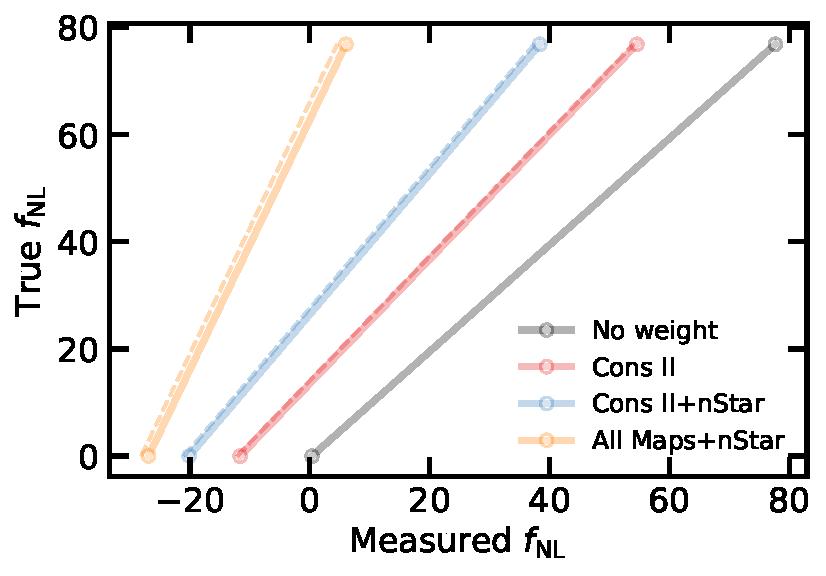
\includegraphics[width=0.45\textwidth]{figures/fnlbias}
\caption{The \textit{No mitigated, clean} vs \textit{mitigated} $\fnl$ values from the $\fnl=0$ and $76.9$ mocks. The solid (dashed) lines represent the best-fitting estimates from fitting the mean power spectrum of the clean (contaminated) mocks. The scatter points show the best-fitting estimates from fitting the individual spectra for the clean mocks.}\label{fig:fnlbias}
\end{figure}


\mr{We find significant shifts in the best-fitting estimates of $\fnl$ from the fits to the mean spectra (summarized in Table \ref{tab:contmocksmcmc}). For $\fnl=0$, we obtain $\Delta \fnl=-12$ for nonlinear three maps, $-20$ for nonlinear three maps, and $-27$ for nonlinear nine maps. Whereas, bigger shifts are noticed for $\fnl=76.9$: we find $\Delta \fnl=-23$ for nonlinear three maps, $-39$ for nonlinear four maps, and $-72$ for nonlinear nine maps. \textbf{MR: TEST with FNL=0 ONLY.}}

To calibrate our methods, we fit a linear curve to the $\fnl$ estimates from the mean power spectrum of the mocks, $f_{\rm NL, no~mitigation, clean} = m_{1} f_{\rm NL, mitigated} + m_{2}$. The $m_{1}$ and $m_{2}$ coefficients for nonlinear three, four, and nine maps are summarized in Table \ref{tab:debiasparams}. These coefficients represent the impact of the cleaning methods on the likelihood. The uncertainty in $\fnl$ after mitigation increases by $m_{1}-1$. Figure \ref{fig:fnlbias} also shows that the choice of our cleaning method can have significant implications for the accuracy of the measured $\fnl$, and careful consideration should be given to the selection of the primary imaging systematic maps and the calibration of the cleaning algorithms in order to minimize systematic uncertainties.


\begin{table}
\begin{center}
\caption{Linear parameters employed to de-bias the $\fnl$ constraints to account for the over-correction issue.}\label{tab:debiasparams}
\begin{tabular}{lcc}
\hline
\hline
\textbf{Cleaning Method} & $m_{1}$ & $m_{2}$ \\
\hline
Nonlinear Three Maps & 1.17 & 13.95 \\
Nonlinear Four Maps & 1.32 & 26.97 \\
Nonlinear Nine Maps & 2.35 & 63.5\\
\hline
\end{tabular}
\end{center}
\end{table}
